\chapter[Usabilidade]{Usabilidade}
Este capítulo tem como foco abordar o tema de usabilidade com a finalidade de responder parcialmente a questão: Quais os métodos de avaliação de serviço permitem a aferição da qualidade de serviços digitizados? 

\section{Definição}

Esta seção define o modelo de qualidade externa e interna. Ele categoriza os atributos de qualidade de software em seis
características (funcionalidade, confiabilidade, usabilidade, eficiência, manutenibilidade e portabilidade) as quais são, por
sua vez, subdivididas em subcaracterísticas (figura 4). As subcaracterísticas podem ser medidas por meio de métricas
externas e internas.
Uma definição é atribuída para cada característica e para cada subcaracterística do software que influencia a característica
de qualidade. A capacidade do software é determinada por um conjunto de atributos internos que podem ser medidos,
para cada característica e subcaracterística. Exemplos de métricas internas são dados na ISO/IEC 9126-3.
As características e subcaracterísticas podem ser medidas externamente pelo grau da capacidade do sistema contendo o
software. Exemplos de métricas externas são dados na ISO/IEC 9126-2.


De acordo com a ISO\cite{iso9126} que regulamenta a qualidade do produto da engenharia de software, na sua primeira parte, define o modelo de qualidade externa e interna de software.No modelo, exemplificado pela Imagem \ref{img:modelodequalidadeiso}, são categorizados os atributos de qualidade de softwares em 6 características:
\begin{itemize}
	\item{Funcionalidade;}
	\item{Confiabilidade;}
	\item{Usabilidade;}
	\item{Eficiência;}
	\item{Manutenibilidade;}
	\item{Portabilidade.}
\end{itemize}

\begin{center}
	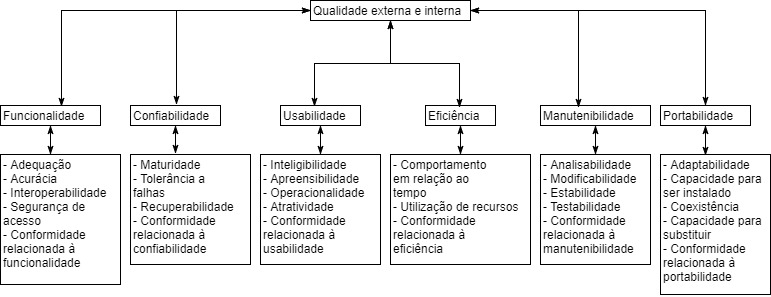
\includegraphics[width=1\linewidth]{figuras/modelodequalidadeiso.jpg}
	\captionof{figure}{Modelo de Qualidade para qualidade externa e interna. Adaptado de \cite{iso9126}}
	\label{img:modelodequalidadeiso}
\end{center}

De todos os atributos listados o que mais se aproxima da visão do usuário sobre o software é a Usabilidade, os outros atributos analisam as características técnicas de construção e manutenção do software, portanto iremos definir como o foco e utilizar para esse trabalho a usabilidade como parâmetro principal para a avaliação.

Ainda de acordo com a norma \cite{iso9126} usabilidade é "a capacidade do produto de software de ser compreendido, aprendido, operado e atraente ao usuário, quando usado sob condições especificadas". Ainda é declarado que alguns aspectos como a funcionalidade, eficiência e confiabilidade também afetam a usabilidade, mas para os propósitos da norma, esses outros aspectos não são classificados como usabilidade.

A seguir são definidos todos os tópicos citados como parte da usabilidade de acordo com a NBR 9126 \cite{iso9126}:
\begin{itemize}
	\item Inteligibilidade: Capacidade do produto de software de possibilitar ao usuário compreender se o software é apropriado e como ele pode ser
usado para tarefas e condições de uso específicas, esse item dependerá da documentaçõ e das impressões iniciais oferecidas pelo software;
	\item Apreensibilidade: Capacidade do produto de software de possibilitar ao usuário aprender sua aplicaçãó;
	\item Operacionalidade: Capacidade do produto de software de possibilitar ao usuário operá-lo e controlá-lo, que corresponde à controlabilidade, tolerancia a erros e conformidade com as expectativas do usuário, como definido na ISO 9241-10;
	\item Atratividade: Capacidade do produto de software de ser atraente ao usuário, que se refere aos atributos de software que possuem a intenção de tornar o software mais atraente para o usuário, como o uso de cores e da natureza do projeto gráfico;
	\item Conformidade relacionada à usabilidade: Capacidade do produto de software de estar de acordo com normas, convenções, guias de estilo ou regulamentações
relacionadas à usabilidade.
\end{itemize}

Usabilidade é uma parte importante da interação humano-computador e compreende uma grande área que será explorada para a obtenção do modelo final de avaliação de serviços. Para avaliação de IHC, \cite{preece2005} descrevem os dois tipos principais: Avaliação formativa, que é realizada em vários pontos do desenvolvimento para checar se o produto está sendo construído de acordo com as necessidades dos usuários e a Avaliação somativa, realizada para verificar a qualidade de um produto finalizado. Para o estudo deste trabalho o foco será na avaliação somativa, visto que os serviços a serem avaliados já existem e são produtos finalizados.

\section{Teste de usabilidade}

\cite{preece2005} em seu trabalho definem os paradigmas de avaliação de IHC:
\begin{itemize}
	\item Rápido e sujo;
	\item Testes de usabilidade;
	\item Estudos de campo;
	\item Avaliação preditiva
\end{itemize}

\cite{diniz2010} ratificam a importância da avaliação e traz a definição que a avaliação somativa, ou conclusiva, é "utilizada para avaliar qualquer objetivo de avaliação". Os autores trazem também a dimensão de localização para o teste, que pode ser definido como avaliação em contexto de uso, onde os testes são realizados onde o usuário costuma usar o sistema a ser avaliado e permite verificar informações do cotidiano e a forma com que o usuário se apropria da tecnologia e quais problemas podem ocorrer em situações reais. A outra opção é realizar os testes em laboratório, onde todas as variáveis são controladas, medidas e observadas, desta forma todos os resultados são de forma pradronizada.

\cite{diniz2010} definem ainda os tipos de métodos de avaliação, que essencialmente são: Inspeção, Investigação e observação de uso. O primeiro permite ao avaliador inspecionar uma solução de IHC para tentar antever as possíveis consequências de decisões sobre as experiencias de uso e geralmente não envolvem diretamente usuários.
Os métodos de investigação usam os questionários, entrevistas, grupos focais e estudo de campo, entre outros. Esses métodos permitem ao avaliador ter acesso, interpretar e consolidar opiniões, expectativas e comportamentos do usuário em relação ao sistema avaliado.
O terceiro método de avaliação, a observação de uso, fornece dados sobre as dificuldades que o usuário enfrenta ao realizar uma tarefa, sendo ela no sistema ou fora, dando insumos para identificar a experiência do usuário e os reais problemas enfrentados.

De posse do tipo de avaliação, paradigma e método de avaliação se fazem necessários definir as atividades básicas para a realização de uma avaliação de usabilidade, os métodos possuem as atividades básicas descritas segundo \cite{diniz2010}:
\begin{itemize}
	\item{Preparação;}
	\item{Coleta de dados;}
	\item{Interpretação;}
	\item{Consolidação;}
	\item{Relato dos resultados.}
\end{itemize}

Na preparação é preciso definir os objetivos e questões específicas de invetigação, o escopo da avaliação, os métodos, os perfis e os números de participantes. Após isso faz-se necessário tratar das questões éticas a serem observadas, alocar recursos e equipamentos bem como a confecção do material de apoio dos testes, realizar um teste-piloto e recrutar participantes.

A coleta de dados vai depender do método e dos objetivos planejados. Utilizará dos itens definidos neste capítulo para coletar os dados e consolidá-los em documentos que se possa analisar.

A interpretação é a análise do material registrado no passo anterior para que se possa atribuir significado a esses dados. Este passo também é dependente do método de avaliação utilizado o que muda o foco da interpretação, mas os métodos costumam apontar suas tendências de interpretação, como por exemplo, o método de avaliação por investigação foca na percepção do usuário do sistema avaliado enquanto o método de inspeção é focado nas tendências de problemas em uso de usuários avaliados por um especialista.

Os resultados individuais são consolidados e analisados em conjunto, tendo como resultado as características representativas de cada grupo e a justificativa das respostas das questões de investigação terem ou não sido respondidas. A generalização dos resultados ocorre nesse passo, mas precisa ser tratada com cautela, pois os dados são fortemente influenciados por características externas à avaliação, como preferências, interesses e necessidades de cada participante.

O último passo é definido pela conclusão da avaliação e a entrega de todos os dados adquiridos durante o processo. Os dados tidos como conclusão nesse passo, indicam uma tendência de problemas e não a certeza que eles irão ocorrer, assim como se não houverem falhas encontradas durante a avaliação, não se pode dizer que o sistema tenha alta qualidade de uso. Portanto o planejamento deve ser personalizado de forma a capturar os melhores dados dentro de um escopo bem definido para a validade do modelo de avaliação.

As características de avaliação de usabilidade aqui descritas serão utilizadas na obtenção do modelo de avaliação de serviços digitizados governamentais, visto que por se tratar de um serviço digitizado a avaliação de usabilidade deve estar presente para tornar o modelo mais robusto e capturar mais características na avaliação pelo usuário.
